\section{Deep Reinforcement Learning}
	In this section we will discuss the content of two developed notebooks, mainly the theory behind Deep Reinforcement Learning (DRL). We will get to know the basic concept of RL, see on an exemplary neural network model the deep learning aspect and work out the necessary formulas in order to translate the theory into code. Further we will introduce a framework, which helps building this project by providing a game to play, more on that later.  All the theory, explanations and code can be viewed in completion in the enclosed notebooks:
	\begin{enumerate}
		\item Deep Reinforcement Learning Beginners Tutorial (1) - Theory 
		\item Deep Reinforcement Learning Beginners Tutorial (2) - Practice
	\end{enumerate}
	
motivation	

\subsection{The Software Agent}
	Befor we start with the topic of RL we have to adress some basics in order to clarify the following explaination. We will use the term of \textit{software agent}, which, as part of artificial intelligence, is a program, that acts self sufficient to solve a task. There are three important aspects an agent should fulfill. First are autonomous actions. An agent needs to make decisions without external help. Further an agent needs to execute multiple actions to complete its task, so it should be proactive. Last but not least, an agent has to be reactive, which means it reacts on changes in the environment it is in. An optional ability for an agent like this is independent improvement. For this the agent builds up knowledge after repetitively doing its task and improves itself this way.\\
	Basically, the part of the agent, which controls its actions, can be filled with different algorithms. In our case, this will be an implementation of RL, which fulfills all requirements of an agent.

\subsection{Reinforcement Learning}
	Reinforcement Learning is considered one of the three machine learning paradigms, alongside supervised learning and unsupervised learning. The main goal of RL is to create an agent, which can navigate by actions in an environment in a way to maximize a representation of a cumulative reward. The evironment is a space that contains the agent. We will talk about the environment later on. In order to miximize the reward, the agent has to learn by trial and error which actions most likely lead to a reward and which lead to a penalty. After some training, the agent will use its knowledge to avoid previous mistakes. It still has to explore the environment, because otherwise we can not be sure if we actually find the global maximum or just a local one and if there might be a better chain of actions. If we think about our real world, this method of learning is pretty close the human learning. If we get hurt for example, we are more likely to try to avoid the situation. Still curiosity or necessity leads us to exploring and thus maybe getting us into danger, but in the best case, will lead us to some kind of positive reward.\\
	
	\subsubsection{The concept of RL}
		Our agent is contained by an environment. A momentary snapshot of the environment is called state. A state contains all information at a certain point in time for example the position of the agent or enemies. There is a permanent exchange of information between the agent and its environment. The agent receives the actual state and has to choose an action based on its logic. Everything the agent can use to alter its environment is called an action. It changes the environment based on a certain set of rules. After executing an action the agents receives the new state and a reward, which helps to decide whether its decision leads to a positive result. Keep in mind, that a reward can also be negative. The main goal for the agent is to learn the best action for each state, so that it can maximize the reward. Basically, an environment is just a set of states. We can move between states by executing actions. A good example for an environment is our own world. We are agents, moving in the world. All the time we have to look at our surroundings and choose an action like moving accross the street or waiting until it is free. The laws of physics restrain us, take gravity for example. We receive rewards like geting hurt oder feeling satisfied, thats how we evalute our actions. Our environment is constantly changing, so we have to reevalute our decisions and choose an action again. The following picture shows the whole procedure:\\ 

		\begin{figure}[h!]
			\begin{center}
				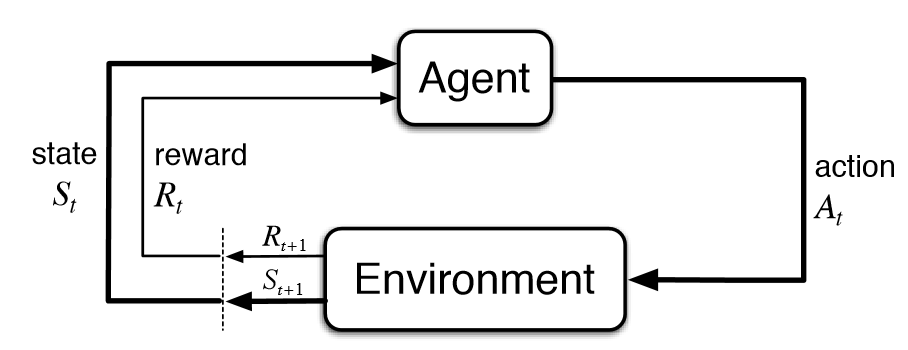
\includegraphics[width=0.6\linewidth]{img/eoeSq.png}
				\caption{Concept of Reinforcement Learning}
				\label{concept}
			\end{center}
		\end{figure}

	\subsubsection{Deep Learning Aspect}
		The agent has to recognize and differentiate elements in the environment, to be able to act accordingly and choose a proper action. In the best case, we already have the input reduced into some important numbers, which describe the actual state. In real applications this may not be possible or feasible with our knowledge. Most of the time we will have a picture available for example the image of a camera or a game screen, but the input we receive can basically be any sensory data.\\
		
		Furthermore the agent must associate the occurence of individual elements on screen with its own actions and the subsequent reward or penalty, which may occur only after several steps in the future. Depending on the situation it may be also necessary to estimate what the next state of the game could be. There are two possible ways to use the Deep Learning aspect.
		
		\begin{enumerate}
			\item Image processing with a Convolutional Neural Network (CNN), in order to process the image information and send this to the agent.
			\item A Deep Q-Learning Network (DQN), in order to model the Q-function, which is discussed below.
		\end{enumerate}
	
		Following is an exemplary presentation of a neural network, which is designed according to the tasks just mentioned.
		
		\begin{figure}[h!]
			\begin{center}
				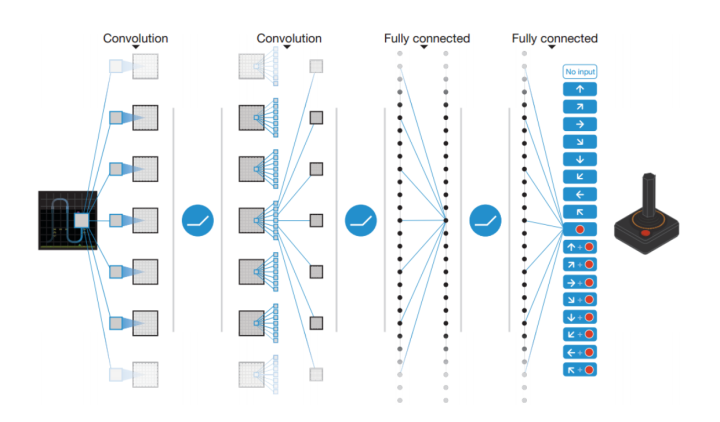
\includegraphics[width=\linewidth]{img/v2-67ef75bb7f5e67b2a42645aa821894bf_hd.png}
				\caption{Concept of Reinforcement Learning}
				\label{concept}
			\end{center}
		\end{figure}

		There are two ways to learn in deep reinforcement learning. Eiher we can use Value Learning or Policy Learning. With Value Learning, we assign values to each state-action pair, which correspond to the probabilities of the pair beeing the best option. In Policy Learning, we will learn a strategy instead, which gives as the best estimated action for a given state s. We will focus at Value Learning. 
			
	\subsubsection{Q-Learning}
		The task of the agent is the maximization of a cumulative future reward. An example of this can be the score in a game. In an environment, there is no guarantee for an immediate reward after executing an action. In many cases, only specific chains of actions lead to a positive reward, so the agent needs to learn multiple moves in succession in order to fulfill the given task. For example, if the agent needs to collect an object in order to get a higher score, it may be necessary to take multiple moves to reach it. The moves in between may not increase the reward significantly or even reduce it, however they are needed to complete the task in order to be successfull. So the agent may have to learn to sacrifice some rewards, to earn an overall higher reward in the end. A simple way to implement RL is Q-Learning. We assign a numerical value to each action we can execute per state. This value is called Q-value. It represents an estimate of which action will result in the highest reward for the actual state. This is the knowledge of our agent. In the beginning all these values are initialized by 0. Each step we have to choose an action for the actual state. This is either random or knowledge based, but all the actions taken, provide data the agent is trained with. We use random actions to explore our environment at first. If we use the knowledge of the agent, the next action is chosen by exploitation, so the agent uses the action with the highest Q-value for the given state. Our next step is the associated function. The Q-function is the name giving aspect of a Deep Q-Learning Network, while the "Q" stands for "Quality". The higher the reward, the higher the estimated Q-value and associated quality. That means this function calculates a Q-value for the actual state, which represents the best action to take. Therefor taking into account the highest Q-value associated with the heighest estimated future total Reward $Q(s', a')$, the last gained reward and a discount factor, in order to make rewards in the near future more dicisive for the agent. The main formula to model such a behaviour is the so called \textit{Bellman equation}.
		
		$Q(s_t, a_t) = r_t + \gamma * \max\limits_{a'} Q(s', a')$
		

\subsection{The OpenAi Gym Framework}
	OpenAi Gym is the Framework we chose to provide an game environment. Developing Machine Learning algorithms is often neither easy to understand nor comprehensible especially for beginners. In order to counteract this, we chose a simple and completly observable environment, in form of a game. OpenAi Gym is open source, so we use it immediately and don't need to spend time or resources to build our own environment. Furthermore the framework provides all environmental data an DRL agent needs and using an existing game is also easier to compare to human performance and therefore the evaluation of different algorithms is easier. 

\subsection{The Exercises}
	The exercises are a comparatively small part of the notebooks. Our main goal is to understand Deep Reinforcement Learning. The places where we want to be active, are designed so that we can translate the theory directly into code, just like that. All other code passages are explained in detail, so that the project can be comprehended in its entirety. The goal of the exercises is to build and understand a basic structure for a DRL agent. The individual tasks are located at the points in the code where the agent can be further optimized and customized to create an entry point into a project.
	   
	
